\subsection{The katz-eig algorithm}\label{sec:background:katzeig}

The \textit{katz-eig} algorithm used is an adaptation \citep{shin2012multi} of a link prediction measure Katz \citep{katz1953new}. Katz is defined as follows, if $A$ is the interaction matrix and the measure is used to produce recommendation predictions

\begin{equation}
    P = \sum_{t=1}^{\infty} \beta^t A^t = (I - \beta A)^{-1} - I
\end{equation}

where $I$ is the identity matrix. The intuition is that for each iteration $t$, one link in the interaction graph defined by user-item pairs is traversed and propagated to introduce transitive connections in the graph. The parameter $\beta \leq \| A \|_2$ represents the link dampening, links far away adds a smaller weight than links closer to the initial node.

The problem with this definition is computational complexity, computing the Katz measure takes $\BigO{n^3}$ time which is not practical for large matrices. This is why the Singular Value Decomposition (SVD) is used.

$A$ can be approximated by a rank $k$ SVD so $A \approx U * S * V^T$. $S$ is a $k$ x $k$ diagonal matrix with the elements representing the $k$ largest singular values. Then the Katz measure can be approximated by

\begin{equation}
    P = \sum_{t=1}^{\infty} \beta^t A^t
    \approx \sum_{t=1}^{\infty} \beta^t (U * S * V^T)^t
    \approx U \left( \sum_{t=1}^{\infty} \beta^t S^t \right) V^T
\end{equation}

Exponentiation is moved from the large interaction matrix $A$ to the small $k$ x $k$ diagonal matrix $S$ which makes the iterative part of the algorithm very fast. Much of the information about the matrix is still contained in $U$ and $V$. The complexity of the algorithm is now on calculating the SVD approximation.

\newpage
Concretely the \textit{katz-eig} algorithm follow these steps:

\begin{enumerate}
    \item Construct $U, S, V$ so $U * S * V^T$ forms a rank $k$ SVD approximation of $A$. Let $S_0 = S$.

    \item At each iteration $t = 1, \ldots, t_{max}$ perform:

        \begin{enumerate}
            \item $S_t = S_{t - 1} + \beta^t * S_{t - 1}^t$
        \end{enumerate}

        Repeat until convergence.

    \item The prediction matrix is given by $P = U * S_{t_{max}} * V^T$.

\end{enumerate}


\subsubsection{Runtime example}

This is a runtime example for \textit{katz-eig} using a simple interaction matrix \eqref{eq:exA_katz}, which is the same matrix as in the example for \textit{link-analysis} (see \sectionref{sec:background:linkanalysis}).

\begin{equation}\label{eq:exA_katz}
  A = \kbordermatrix{
    &    i_1 & i_2 & i_3 & i_4 \\
    u_1 & 0   & 1   & 0   & 1  \\
    u_2 & 0   & 1   & 1   & 1  \\
    u_3 & 1   & 0   & 1   & 0
  }
\end{equation}

This example uses $K = 2$, $\beta = 0.1$ and is run for $t_{max} = 3$ iterations.

Firstly a rank 2 SVD approximation is created
\[
U = \begin{pmatrix}
    -0.5592 &  0.4472 \\
    -0.7805 &  0.0000 \\
    -0.2796 & -0.8944 \\
\end{pmatrix},
\;
S = \begin{pmatrix}
    2.1889  &      0 \\
         0  & 1.4142
\end{pmatrix},
\;
V = \begin{pmatrix}
   -0.1277 & -0.6325 \\
   -0.6120 &  0.3162 \\
   -0.4843 & -0.6325 \\
   -0.6120 &  0.3162
\end{pmatrix}
\]

\[
    U * S * V^T = \begin{pmatrix}
       -0.2436 &  0.9491  & 0.1928 &  0.9491 \\
        0.2182 &  1.0455  & 0.8273 &  1.0455 \\
        0.8782 & -0.0254  & 1.0964 & -0.0254
    \end{pmatrix}
    \approx
    A = \begin{pmatrix}
        0   & 1   & 0   & 1 \\
        0   & 1   & 1   & 1 \\
        1   & 0   & 1   & 0
    \end{pmatrix}
\]

Notable here is that some valid recommendations could be made directly from the approximation matrix. In fact for this example there would be no difference in recommendations if $t_{max} = 0$ and the approximation matrix was used directly.

Intuitively a matrix approximation blurs together similar users and items. In a rank $k$ matrix approximation the value of $k$ specifies the blurring degree, the higher $k$ the more of the original matrix will be retained.

\newpage
Initially $S_0$ = $S$. Then $S_t$ is calculated iteratively
\[
    S_1 = \begin{pmatrix}
        0.2189 &    0 \\
        0      & 0.1414
    \end{pmatrix},
    \;
    S_2 = \begin{pmatrix}
        0.2668 &    0 \\
        0      & 0.1614
    \end{pmatrix},
    \;
    S_3 = \begin{pmatrix}
        0.2773 &    0 \\
        0      & 0.1642
    \end{pmatrix}
\]

until convergence or as in our case $t_{max} = 3$. The recommendations are then given by
\[
    U * S_3 * V^T = \kbordermatrix{
        &    i_1 & i_2 & i_3 & i_4 \\
        u_1 &   -0.0266 &  0.1181 &  0.0286 &  0.1181 \\
        u_2 &    0.0276 &  0.1324 &  0.1048 &  0.1324 \\
        u_3 &    0.1028 &  0.0010 &  0.1305 &  0.0010
    }
\]

%\newpage
After removing the items users already have interacted with in $A$, the prediction matrix $P$ becomes
\[
    P = \kbordermatrix{
        &    i_1 & i_2 & i_3 & i_4 \\
        u_1 &   -0.0266 &  0      &  \mathbf{0.0286} &  0      \\
        u_2 &    \mathbf{0.0276} &  0      &  0      &  0      \\
        u_3 &    0      &  \mathbf{0.0010} &  0      &  \mathbf{0.0010}
    }
\]

\Figureref{fig:ex_graph_katz_rec} is a visualization of $P$ displaying the single most recommended item for each user.

\begin{figure}[h!]
    \centering
    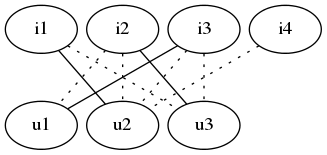
\includegraphics[width=0.3\linewidth]{fig/example_run/item_user_graph_katz_rec.png}
    \caption{A graph representing the most recommended item for each user. The dotted lines represent the interaction history.}
    \label{fig:ex_graph_katz_rec}
\end{figure}

\FloatBarrier

